量子场论的一般有效场论母式在标准模型场内容上的专门化由\eqnrefs{eq:smeft-specialization-dp42} 给出。六维匹配还需要把同一重尺度写成物理四动量的量纲，因此定义匹配动量尺度
\begin{equation}
\boxed{\mu_{\rm M}\equiv\hbar\Lambda_*=\frac{\Lambda_E}{c}},
\qquad [\mu_{\rm M}]=\mathrm{kg\,m\,s^{-1}}.
\label{eq:smeft-matching-momentum-dp13}
\end{equation}
于是逆长度、动量与能量分别由 $\Lambda_*$、$\mu_{\rm M}$ 与 $\Lambda_E$ 表示，不会在对数或重整化群方程中混用。配合 $\widehat\Phi=\Phi/\sqrt{\hbar c}$、$[\psi]=\mathrm{m^{-3/2}}$ 与 $[\mathscr C_\mu]=\mathrm{m^{-1}}$，\eqnrefs{eq:smeft-specialization-dp42} 在 $d=6$ 时给出

若 $\widehat{\mathcal O}_i^{(6)}$ 的几何量纲为 $\mathrm{m^{-6}}$，则
\begin{align}
\Delta\widehat\Lag_6
&=\sum_i\frac{C_i^{(6)}}{\Lambda_*^2}\widehat{\mathcal O}_i^{(6)},
\label{eq:smeft-geometric-normalization-dp13}\\
\Delta\Lag_6
&=\frac{(\hbar c)^3}{\Lambda_E^2}
\sum_iC_i^{(6)}\widehat{\mathcal O}_i^{(6)}.
\label{eq:smeft-si-normalization-dp13}
\end{align}
因此 $C_i^{(6)}$ 全部无量纲。例如 $\widehat{\mathcal O}_H=(\widehat\Phi^\dagger\widehat\Phi)^3$ 对应
\begin{equation*}
\Delta\Lag_H=\frac{C_H}{\Lambda_E^2}(\Phi^\dagger\Phi)^3,
\end{equation*}
单位为 $\mathrm{J\,m^{-3}}$。该几何归一化仅重排幂次计数，所有系数继续保持上述 SI 量纲。


匹配的精确定义是把重场 $H$ 在保持轻场 $\ell$ 外部背景的条件下积分掉：
\begin{equation}
\boxed{
\exp\!\left[\frac{\ii}{\hbar}\Gamma_{\rm LE}[\ell]\right]
=\int\mathcal D H\,
\exp\!\left[\frac{\ii}{\hbar}S_{\rm UV}[\ell,H]\right].}
\label{eq:smeft-matching-functional-dp32}
\end{equation}
该泛函积分定义精确而一般非局域的低能作用量；只有在外部不变量远小于重质量后，对重传播子作预解式展开，才得到局域算符级数。分块二次核\eqnrefs{eq:sm-heavy-block-schur-matching-dp85} 给出一般 Schur 母式。对线性源耦合的二次重场块
\begin{equation*}
\widehat\Lag_{\rm UV}
=\widehat\Lag_{\rm light}+\frac12H\mathsf K_HH+H\mathcal J[\ell],
\end{equation*}
重场方程 $\mathsf K_HH+\mathcal J=0$ 给出 $H_{\rm cl}=-\mathsf K_H^{-1}\mathcal J$；代回二次型，树级低能项立即成为
\begin{equation}
\boxed{
\Delta\widehat\Lag_{\rm LE}^{\rm tree}
=-\frac12\mathcal J\mathsf K_H^{-1}\mathcal J.}
\label{eq:smeft-tree-resolvent-dp32}
\end{equation}
若 $\mathsf K_H=\Lambda_*^2+\mathsf D$，并且在所考察低能态空间内 $\|\mathsf D\|/\Lambda_*^2\ll1$，则重传播子的逆算符可按无量纲小量 $\mathsf D/\Lambda_*^2$ 展开：
\begin{equation}
\boxed{
\mathsf K_H^{-1}
=\frac1{\Lambda_*^2}
\left[
 I-\frac{\mathsf D}{\Lambda_*^2}
 +O\!\left(\frac{\mathsf D^2}{\Lambda_*^4}\right)
\right],
\qquad
\epsilon_{\rm EFT}
\sim\frac{E_{\rm inv}^2}{\Lambda_E^2}\ll1.}
\label{eq:smeft-heavy-resolvent-expansion-dp76}
\end{equation}
第一项产生六维局域算符，下一项产生多两个导数的八维结构，因此有效场论的局域截断就是重传播子的受控低能展开。这里的 $\epsilon_{\rm EFT}\sim E_{\rm inv}^2/\Lambda_E^2$ 是二阶微分重块的具体幂次计数；它是一般控制量\eqnrefs{eq:sm-heavy-field-local-control-dp85} 在该传播子结构下的特化。

\begin{figure}[htbp]
\centering
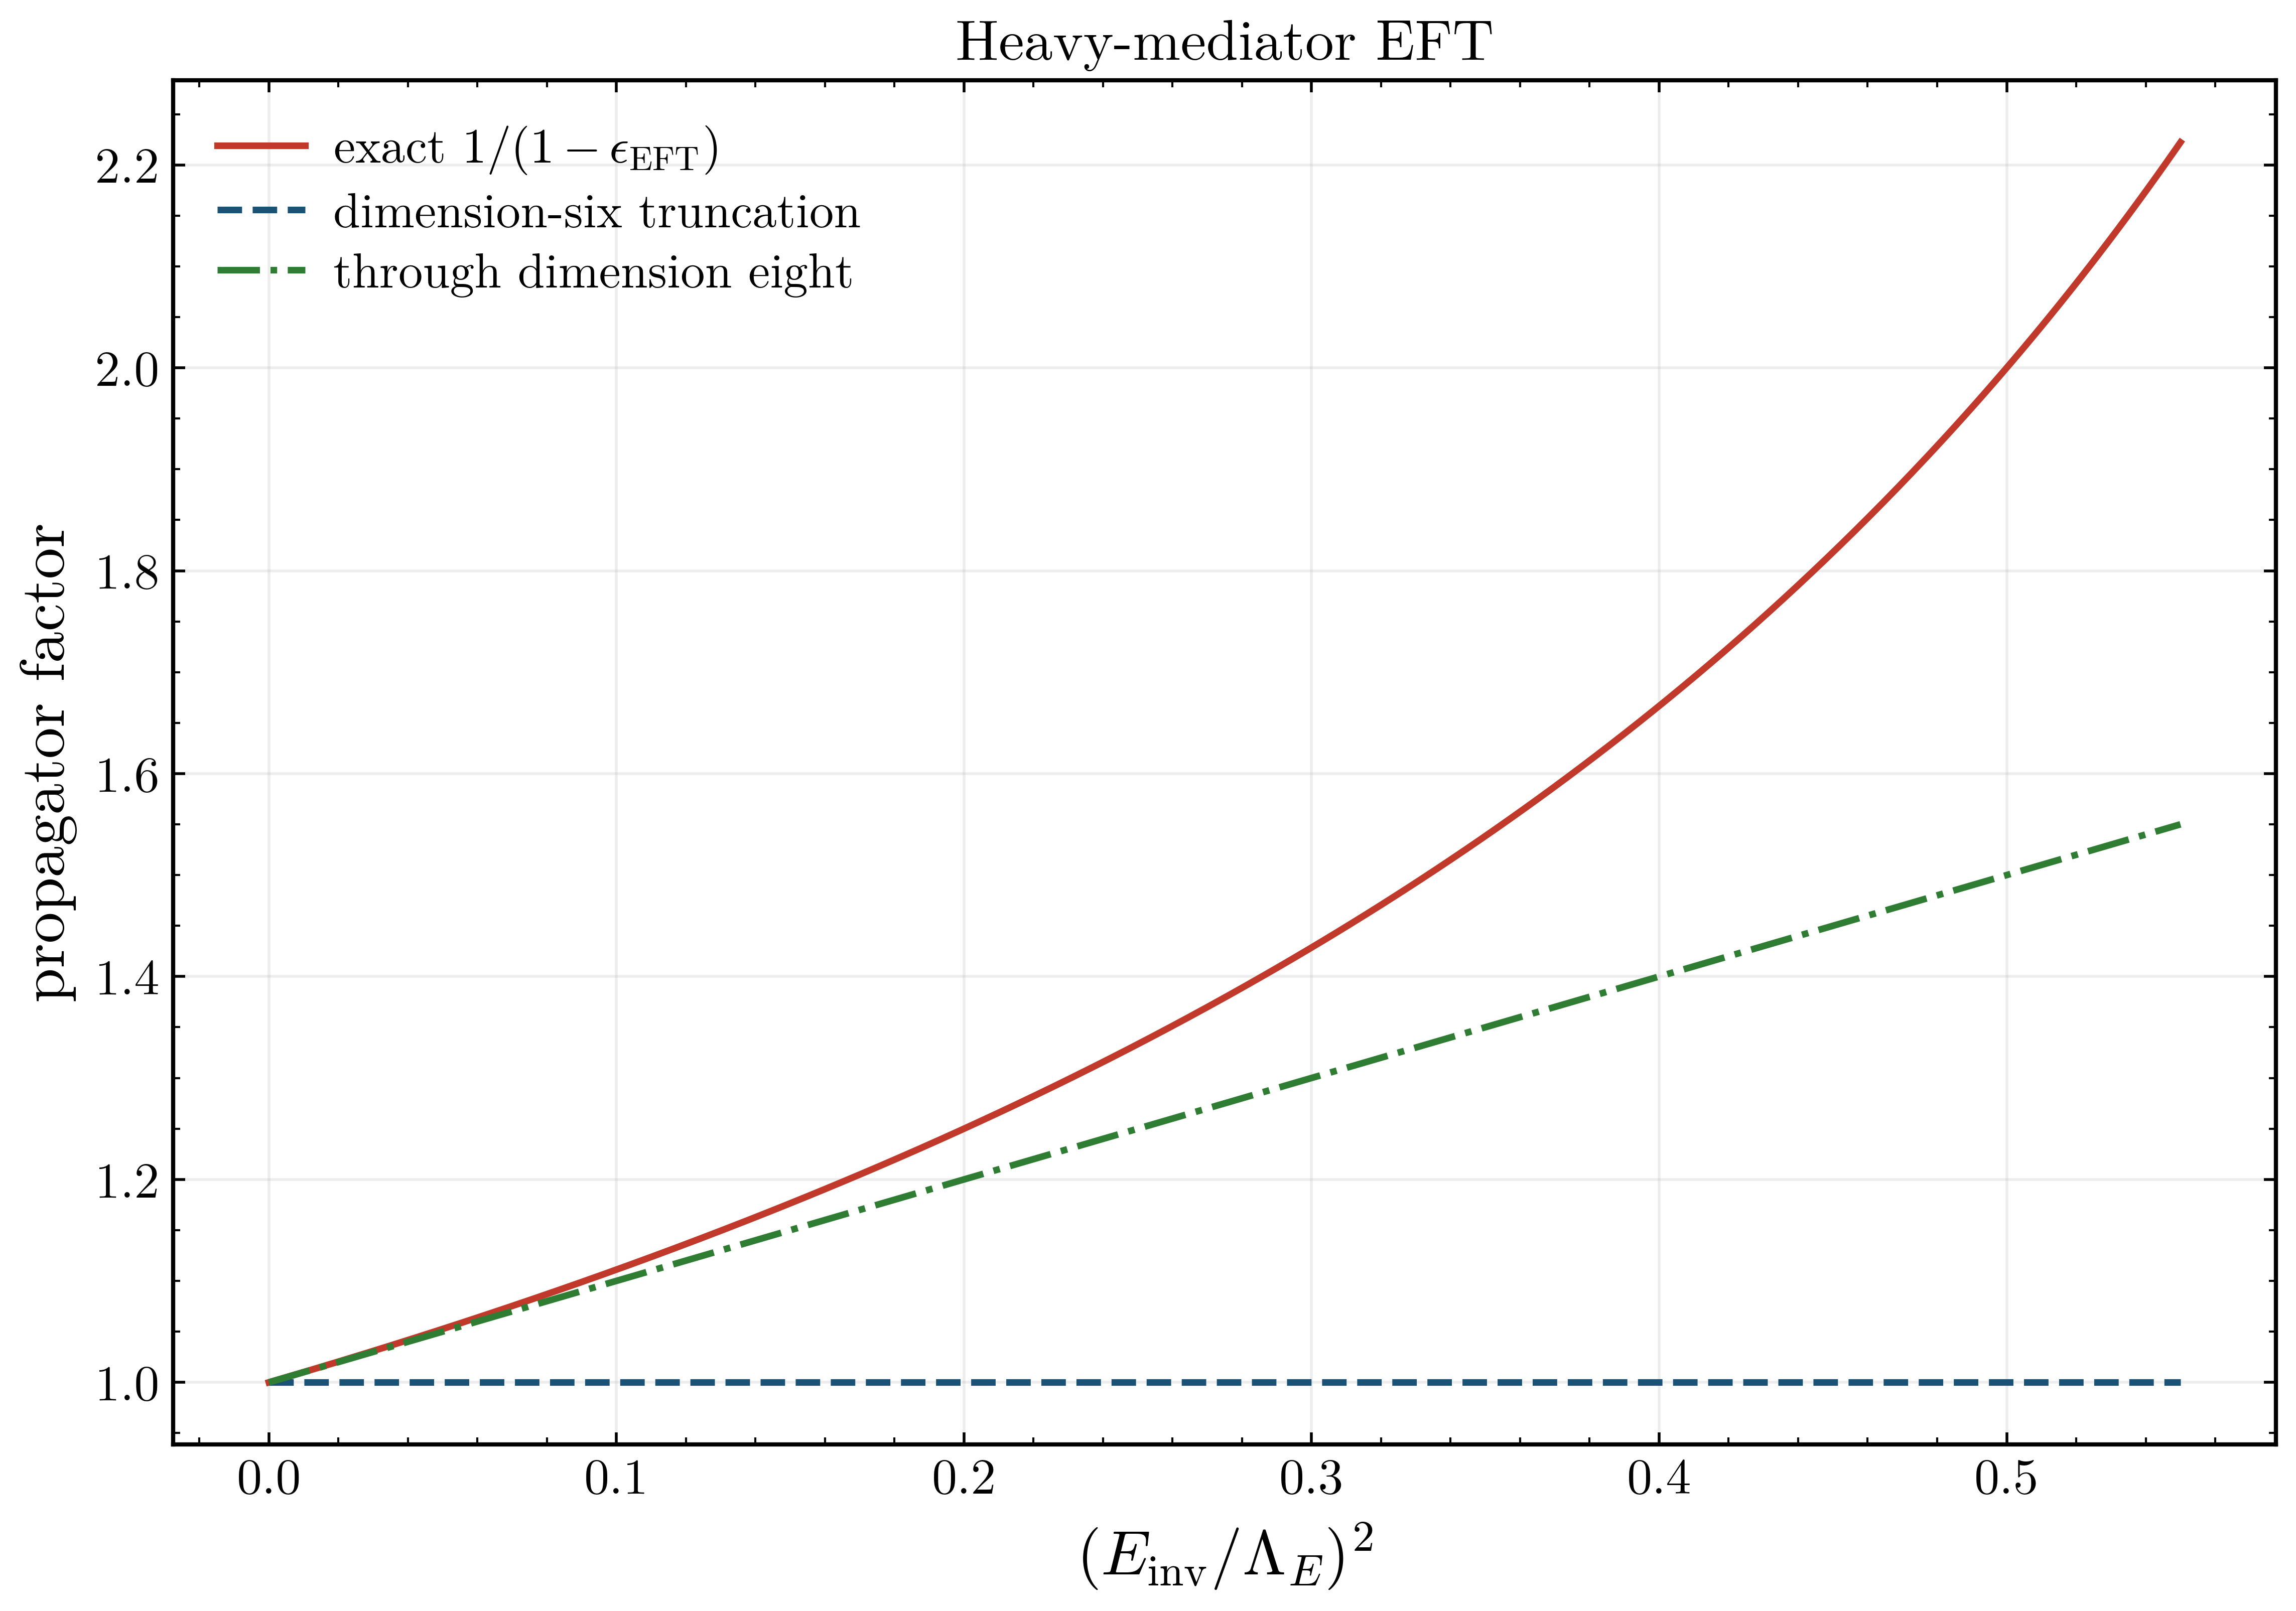
\includegraphics[width=.76\linewidth]{content/FreeElectronQuantumOptics/figures/generated/smeft_propagator_expansion_dp13.png}
\caption{重传播子的局域展开。六维截断只保留预解式的第一项；加入八维项后恢复首个 $E_{\rm inv}^2/\Lambda_E^2$ 修正。随着 $E_{\rm inv}/\Lambda_E$ 增大，有限阶局域展开逐渐失去精度。}
\label{fig:smeft-propagator-expansion-dp13}
\end{figure}

\begin{exbox}[重单态矢量场的树级匹配]
考虑质量尺度为 $\Lambda_*$ 的实矢量场 $X_\mu$，它只耦合到两个标准模型规范单态流
\begin{equation*}
J_L^\mu\equiv\bar L\gamma^\mu L,
\qquad
J_Q^\mu\equiv\bar Q\gamma^\mu Q,
\end{equation*}
并取
\begin{equation}
\widehat\Lag_X
=-\frac14X_{\mu\nu}X^{\mu\nu}
+\frac12\Lambda_*^2X_\mu X^\mu
-X_\mu(g_LJ_L^\mu+g_QJ_Q^\mu).
\label{eq:heavy-vector-uv-lag-dp13}
\end{equation}
记
\begin{equation*}
J_X^\mu\equiv g_LJ_L^\mu+g_QJ_Q^\mu.
\end{equation*}
对 $X_\mu$ 变分得到经典场方程。对守恒外流，纵向传播部分不贡献最低阶局域匹配；在动量空间只需保留横向块，于是
\begin{equation*}
\left(\Lambda_*^2-\frac{q^2}{\hbar^2}\right)X^\mu(q)=J_X^\mu(q),
\end{equation*}
从而
\begin{equation*}
X^\mu(q)
=\frac{J_X^\mu(q)}{\Lambda_*^2-q^2/\hbar^2}
=\frac{J_X^\mu(q)}{\Lambda_*^2}
\left[1+O\!\left(\frac{E_{\rm inv}^2}{\Lambda_E^2}\right)\right].
\end{equation*}
当 $E_{\rm inv}\ll\Lambda_E$ 时，把最低阶经典解 $X^\mu\simeq J_X^\mu/\Lambda_*^2$ 代回二次项与源项：
\begin{align*}
\frac12\Lambda_*^2X_\mu X^\mu-X_\mu J_X^\mu
&=\frac{1}{2\Lambda_*^2}J_{X\mu}J_X^\mu
-\frac{1}{\Lambda_*^2}J_{X\mu}J_X^\mu\\
&=-\frac{1}{2\Lambda_*^2}J_{X\mu}J_X^\mu.
\end{align*}
再展开流的平方，
\begin{align*}
J_{X\mu}J_X^\mu
&=(g_LJ_{L\mu}+g_QJ_{Q\mu})
  (g_LJ_L^\mu+g_QJ_Q^\mu)\\
&=g_L^2J_{L\mu}J_L^\mu
 +2g_Lg_QJ_{L\mu}J_Q^\mu
 +g_Q^2J_{Q\mu}J_Q^\mu.
\end{align*}
因此六维低能拉氏量中的三个四费米子结构分别得到
\begin{equation*}
\Delta\widehat\Lag_6
=\frac1{\Lambda_*^2}
\left[
-\frac{g_L^2}{2}J_L^2
-g_Lg_QJ_L\!\cdot J_Q
-\frac{g_Q^2}{2}J_Q^2
\right]
+O\!\left(\frac{E_{\rm inv}^2}{\Lambda_E^2}\right),
\end{equation*}
所以匹配尺度上的无量纲 Wilson 系数为
\begin{equation}
\boxed{
C_{\ell\ell}^{(1)}=-\frac{g_L^2}{2},
\qquad
C_{\ell q}^{(1)}=-g_Lg_Q,
\qquad
C_{qq}^{(1)}=-\frac{g_Q^2}{2}.}
\label{eq:heavy-vector-wilson-matching-dp13}
\end{equation}
三个系数不是三个任意参数：一个重矢量只提供 $g_L$、$g_Q$ 两个耦合，因此它们满足
\begin{equation*}
\bigl(C_{\ell q}^{(1)}\bigr)^2
=4C_{\ell\ell}^{(1)}C_{qq}^{(1)}.
\end{equation*}
这个关系给出了可直接用于低能拟合的模型检验；若实验提取的三个 Wilson 系数显著不满足它，就不能由这一单一重矢量在树级独自解释。
\end{exbox}

树级匹配并不是唯一来源。如果重实标量 $S$ 通过 $\kappa S^2(\widehat\Phi^\dagger\widehat\Phi)/2$ 与 Higgs 耦合，而且树级经典解为 $S=0$，那么 $\mathcal O_H=(\Phi^\dagger\Phi)^3$ 的第一项从一圈泛函行列式产生。按\eqnrefs{eq:smeft-geometric-normalization-dp13} 的归一化，匹配尺度上的结果为
\begin{equation}
\boxed{
C_H(\mu_{\rm M})=-\frac{\kappa^3}{192\pi^2}.}
\label{eq:heavy-scalar-ch-loop-dp32}
\end{equation}
这里 $1/(16\pi^2)$ 的环抑制和 $1/\Lambda_E^2$ 的局域展开抑制是两个独立层级；不能用一个“有效场论小参数”同时代表二者。

匹配只固定某一尺度上的 Wilson 系数。先把复合算符的重整化混合定义为
\begin{equation}
 \mu_{\rm DR}\frac{\dd\widehat{\mathbf O}}{\dd\mu_{\rm DR}}
 =-\gamma^{\mathcal O}\widehat{\mathbf O}.
 \label{eq:smeft-operator-rg-dp68}
\end{equation}
物理有效拉格朗日量中的组合 $\mathbf C^T\widehat{\mathbf O}$ 不能依赖辅助尺度，因此系数向量必须按相反的转置矩阵作用运行：
\begin{equation}
\boxed{
\mu_{\rm DR}\frac{\dd\mathbf C}{\dd\mu_{\rm DR}}
=(\gamma^{\mathcal O})^T\mathbf C.}
\label{eq:smeft-wilson-rg-dp32}
\end{equation}
当不同尺度上的反常维数矩阵不彼此对易时，不能把它们当成一个常矩阵直接指数化。令 $t=\ln\mu_{\rm DR}$，从匹配尺度 $\mu_{\rm M}$ 演化到任意低能尺度的形式解为
\begin{equation}
\boxed{
\mathbf C(\mu_{\rm DR})
=\mathcal P\exp\!\left[
\int_{\ln\mu_{\rm M}}^{\ln\mu_{\rm DR}}\dd\ell\,
(\gamma^{\mathcal O}(\ell))^T
\right]\mathbf C(\mu_{\rm M}),}
\label{eq:smeft-wilson-evolution-dp90}
\end{equation}
其中 $\mathcal P$ 按尺度参数 $\ell$ 排序；只有当 $[(\gamma^{\mathcal O}(\ell_1))^T,(\gamma^{\mathcal O}(\ell_2))^T]=0$ 时，路径有序符号才可以去掉。
因此某个系数在匹配尺度上为零，并不意味着它在实验尺度上仍为零；只要反常维数矩阵存在非对角元，运行就会生成与原算符发生混合的其他系数。这也是低能算符子空间必须对重整化闭合的原因。

Weinberg 算符的一圈重整化同时涉及普适缩放和味非普适混合。沿用\eqnrefs{eq:sm-higgs-quartic-beta-dp93} 前已经定义的味普适迹 $\mathcal T_Y$，这里只需再定义作用在左手轻子二重态味空间的矩阵
\begin{equation*}
 \mathcal Y_L\equiv Y_eY_e^\dagger.
\end{equation*}
这个左右次序由 Yukawa 项 $\bar L_LY_e\Phi e_R$ 的指标位置固定；$\mathcal T_Y$ 则继续表示全部标准模型 Yukawa 耦合对 Higgs 波函数重整化产生的味普适迹。取 $d=4-2\epsilon$，由于\eqnrefs{eq:weinberg-operator-dp11} 含两个 $L_L$ 和两个 $\Phi$ 外腿，裸系数与重整化系数的矩阵关系必须写成
\begin{equation}
\boxed{
 C_B^{(5)}
 =\mu_{\rm DR}^{2\epsilon} Z_\Phi^{-1}
 (Z_L^T)^{-1/2}
 \left[C^{(5)}+\delta C^{(5)}\right]
 Z_L^{-1/2}.}
\label{eq:weinberg-bare-renorm-dp91}
\end{equation}
这里 $Z_L$ 是左手轻子二重态的味空间波函数重整化矩阵，$Z_\Phi$ 是 Higgs 二重态的波函数重整化常数，$\delta C^{(5)}$ 是四点 1PI 顶角的局域反项。矩阵因子的左右次序不能交换；它正是 Weinberg 系数保持复对称性的原因。

在 $Q=T_3+Y$ 的超荷约定和\eqnrefs{eq:sm-higgs-lagrangian-dp11} 的 Higgs 势
$V=-\mu_H^2\Phi^\dagger\Phi+\lambda_H(\Phi^\dagger\Phi)^2/(\hbar c)$ 归一化下，一圈标准模型运行最终为
\begin{align}
16\pi^2\mu_{\rm DR}\frac{\dd C^{(5)}}{\dd\mu_{\rm DR}}
={}&\left[4\lambda_H-3g^2+2\mathcal T_Y\right]C^{(5)}\nonumber\\
&-\frac32\left[\mathcal Y_L^T C^{(5)}+C^{(5)}\mathcal Y_L\right].
\label{eq:weinberg-matrix-rg-dp32}
\end{align}
$4\lambda_H-3g^2+2\mathcal T_Y$ 只改变味矩阵的整体缩放；$\mathcal Y_L^TC^{(5)}+C^{(5)}\mathcal Y_L$ 则沿带电轻子 Yukawa 的左手味方向产生非普适形变。因而跨越很大的能标区间时，中微子质量的整体尺度和 PMNS 参数都可能运行。

\begin{figure}[htbp]
\centering
\begin{tikzpicture}[>=Latex,node distance=13mm and 14mm,line label/.style={fill=white,fill opacity=.96,text opacity=1,inner sep=1.15pt}]
\node[draw,rounded corners,align=center,minimum width=34mm,minimum height=13mm] (uv) {UV theory\\light $+$ heavy fields};
\node[draw,rounded corners,align=center,right=of uv,minimum width=31mm,minimum height=13mm] (match) {threshold matching\\$E\sim\Lambda_E$};
\node[draw,rounded corners,align=center,right=of match,minimum width=34mm,minimum height=13mm] (wilson) {$C_i(\Lambda_E)$\\local operators};
\node[draw,rounded corners,align=center,below=of wilson,minimum width=34mm,minimum height=13mm] (rg) {$\gamma_{ij}$\\operator mixing};
\node[draw,rounded corners,align=center,left=of rg,minimum width=31mm,minimum height=13mm] (low) {$C_i(E)$\\experimental scale};
\node[draw,rounded corners,align=center,left=of low,minimum width=34mm,minimum height=13mm] (obs) {observable\\SM $+$ EFT};
\draw[->,thick] (uv)--node[line label,midway,above,font=\scriptsize]{integrate out heavy modes}(match);
\draw[->,thick] (match)--node[line label,midway,above,font=\scriptsize]{boundary conditions}(wilson);
\draw[->,thick] (wilson)--node[line label,midway,right,font=\scriptsize]{anomalous dimensions}(rg);
\draw[->,thick] (rg)--node[line label,midway,below,font=\scriptsize]{RG evolution / log resummation}(low);
\draw[->,thick] (low)--(obs);
\end{tikzpicture}
\caption{有效场论的单向计算链。高能阈值决定匹配条件，算符反常维数矩阵把 Wilson 系数运行到实验尺度，最后才与低能矩阵元组合成可观测量。}
\label{fig:smeft-matching-running-chain-dp13}
\end{figure}

局域截断由 $\epsilon_{\rm EFT}=E_{\rm inv}^2/\Lambda_E^2\ll1$ 控制；匹配的环截断由 $g_*^2/(16\pi^2)$、$g_s^2/(16\pi^2)$ 等参数控制；重整化群截断则由反常维数的环展开控制。若 $|\ln(\Lambda_E/E)|\gg1$，即使耦合很小，固定阶中的 $g^2\ln(\Lambda_E/E)/(16\pi^2)$ 也可能达到一阶，此时必须在高能阈值先做匹配，再用重整化群重求和到实验尺度。


标准模型有效场论的计算顺序由四个彼此不同的步骤组成：重场泛函积分定义低能作用量；低能展开把非局域传播子转成局域算符；匹配固定高能阈值处的 Wilson 系数；算符混合再把这些系数运行到实验尺度。树级重矢量场展示了系数相关性，一圈重标量展示了独立的环抑制，Weinberg 算符则展示了真实味矩阵的重整化群形变。

